\section{On-chain Protocol}\label{sec:mainchain}

We describe the details of the \emph{on-chain} protocol controlling a
Hydra head (see Fig.~\ref{fig:SM_states_basic}) using the CEM abstraction \&
notation (see Section~\ref{sec:cem}). In addition of standard CEM modeling, we
also provide the formal conditions $\cemTxCon$ which a transition need to
satisfy and also include them in the accompanying text.

The following sections describe the structure of each of the transactions comprising 
the Head protocol: Initial, Commit, Abort, CollectCom, Close, Contest, and FanOut. 
Following the eUTxO model, this structure is enforced on-chain through \emph{validators}, eg. scripts attached to each UTxO run as part of the ledger's validation. 

\todo{explain how scripts/contracts relate to this}

% TODO: no generic OCV anymore
% \dparagraph{Onchain verification algorithms.} The status of the head
% is maintained in a variable $\eta$, which is part of the SM state and
% updated by so-called \emph{onchain verification (OCV) algorithms}
% $\ocvInitial$, $\ocvClose$, $\ocvContest$, and $\ocvFinal$. In the context
% of the mainchain protocol, these OCV algorithms are intentionally kept
% as generic as possible; this keeps the mainchain SM compatible with
% many potential head-protocol variants.
% The concrete OCV algorithms for the head protocol specified in this
% paper are given in context of the head protocol itself as they depend
% on the specific head-protocol internals: verification of head-protocol
% certificates and related onchain state updates.
% As such, the OCV algorithms can be seen as abstract mainchain algorithms
% implemented by the specific head protocol. Consequently, the OCV
% implementation for our head protocol is described in Section~\ref{sec:hpocv}.

\subsection{Initial transaction} 

The \mtxInit{} transaction (see
Fig.~\ref{fig:SM_commit_tx}) establishes the initial state of the protocol as the tuple
$$
(\stInitial,\hpAK,\hppuv,\nop,\cPer)
$$ 
where:
\begin{menumerate}
    \item $\stInitial$ is
a state identifier, 
   \item $\hpAK$ is the aggregated multi-signature key established
during the setup phase, 
  \item $\hppuv$ is the list of all participants verification
keys $(k_1,\ldots,k_\nop)$ exchanged during the setup phase and identifying the
head members, 
  \item $\nop$ is the number of head members, and 
  \item $\cPer$ is the length of the contestation period.
\end{menumerate} 

\subsubsection{Head Tokens}

The \mtxInit{} transaction also mints tokens whose \emph{Minting Policy} is $\mathsf{cid}$, defined as 
$$
\mathsf{cid} = H(\muHead(\mathsf{tx_{in}})),
$$
where $\mathsf{tx_{in}}$ is one of the inputs spent in the \mtxInit{} transaction. From the ledger preventing double-spending and the uniqueness of $\mathsf{tx_{in}}$, $\mathsf{cid}$ is guaranteed to be unique and can be used to identify the newly initialized head. \\
\\
Two kinds of tokens are minted:
\begin{itemize}
\item $\mathsf{ST}$: A single \emph{State Thread} token marking the output carrying the state of the protocol on-chain, whose name is the well known string \texttt{HydraHeadV1},
\item $\mathsf{PT}_i,\ i\in \{1 \dots \nop \}$: One participation token per participant, where the token name is the participant's verification key hash $H(k_i)$. This will be used to authenticate participants in protocol transactions.
\end{itemize}

\subsubsection{Initial Outputs}

The \mtxInit{} transaction has $\nop$ outputs, where each output is
locked by validator $\nuInitial$ and the $\ith i$ output has the participation
token $\mathsf{PT}_i$ in its value, and $\mathsf{cid}$ as a datum. Validator $\nuInitial$
ensures that the output is consumed by either by \mtxAbort{} (see section \ref{sec:abort-tx} below) or \mtxCom{} (see section \ref{sec:commit-tx} below).

The general well-formedness and validity of the \mtxInit{} transaction is
checked on the mainchain. The head members can additionally check whether the head
parameters match the parameters agreed on during the setup phase.

\subsection{Commit Transaction}\label{sec:commit-tx}

\begin{figure}[h]

  \centering

  % 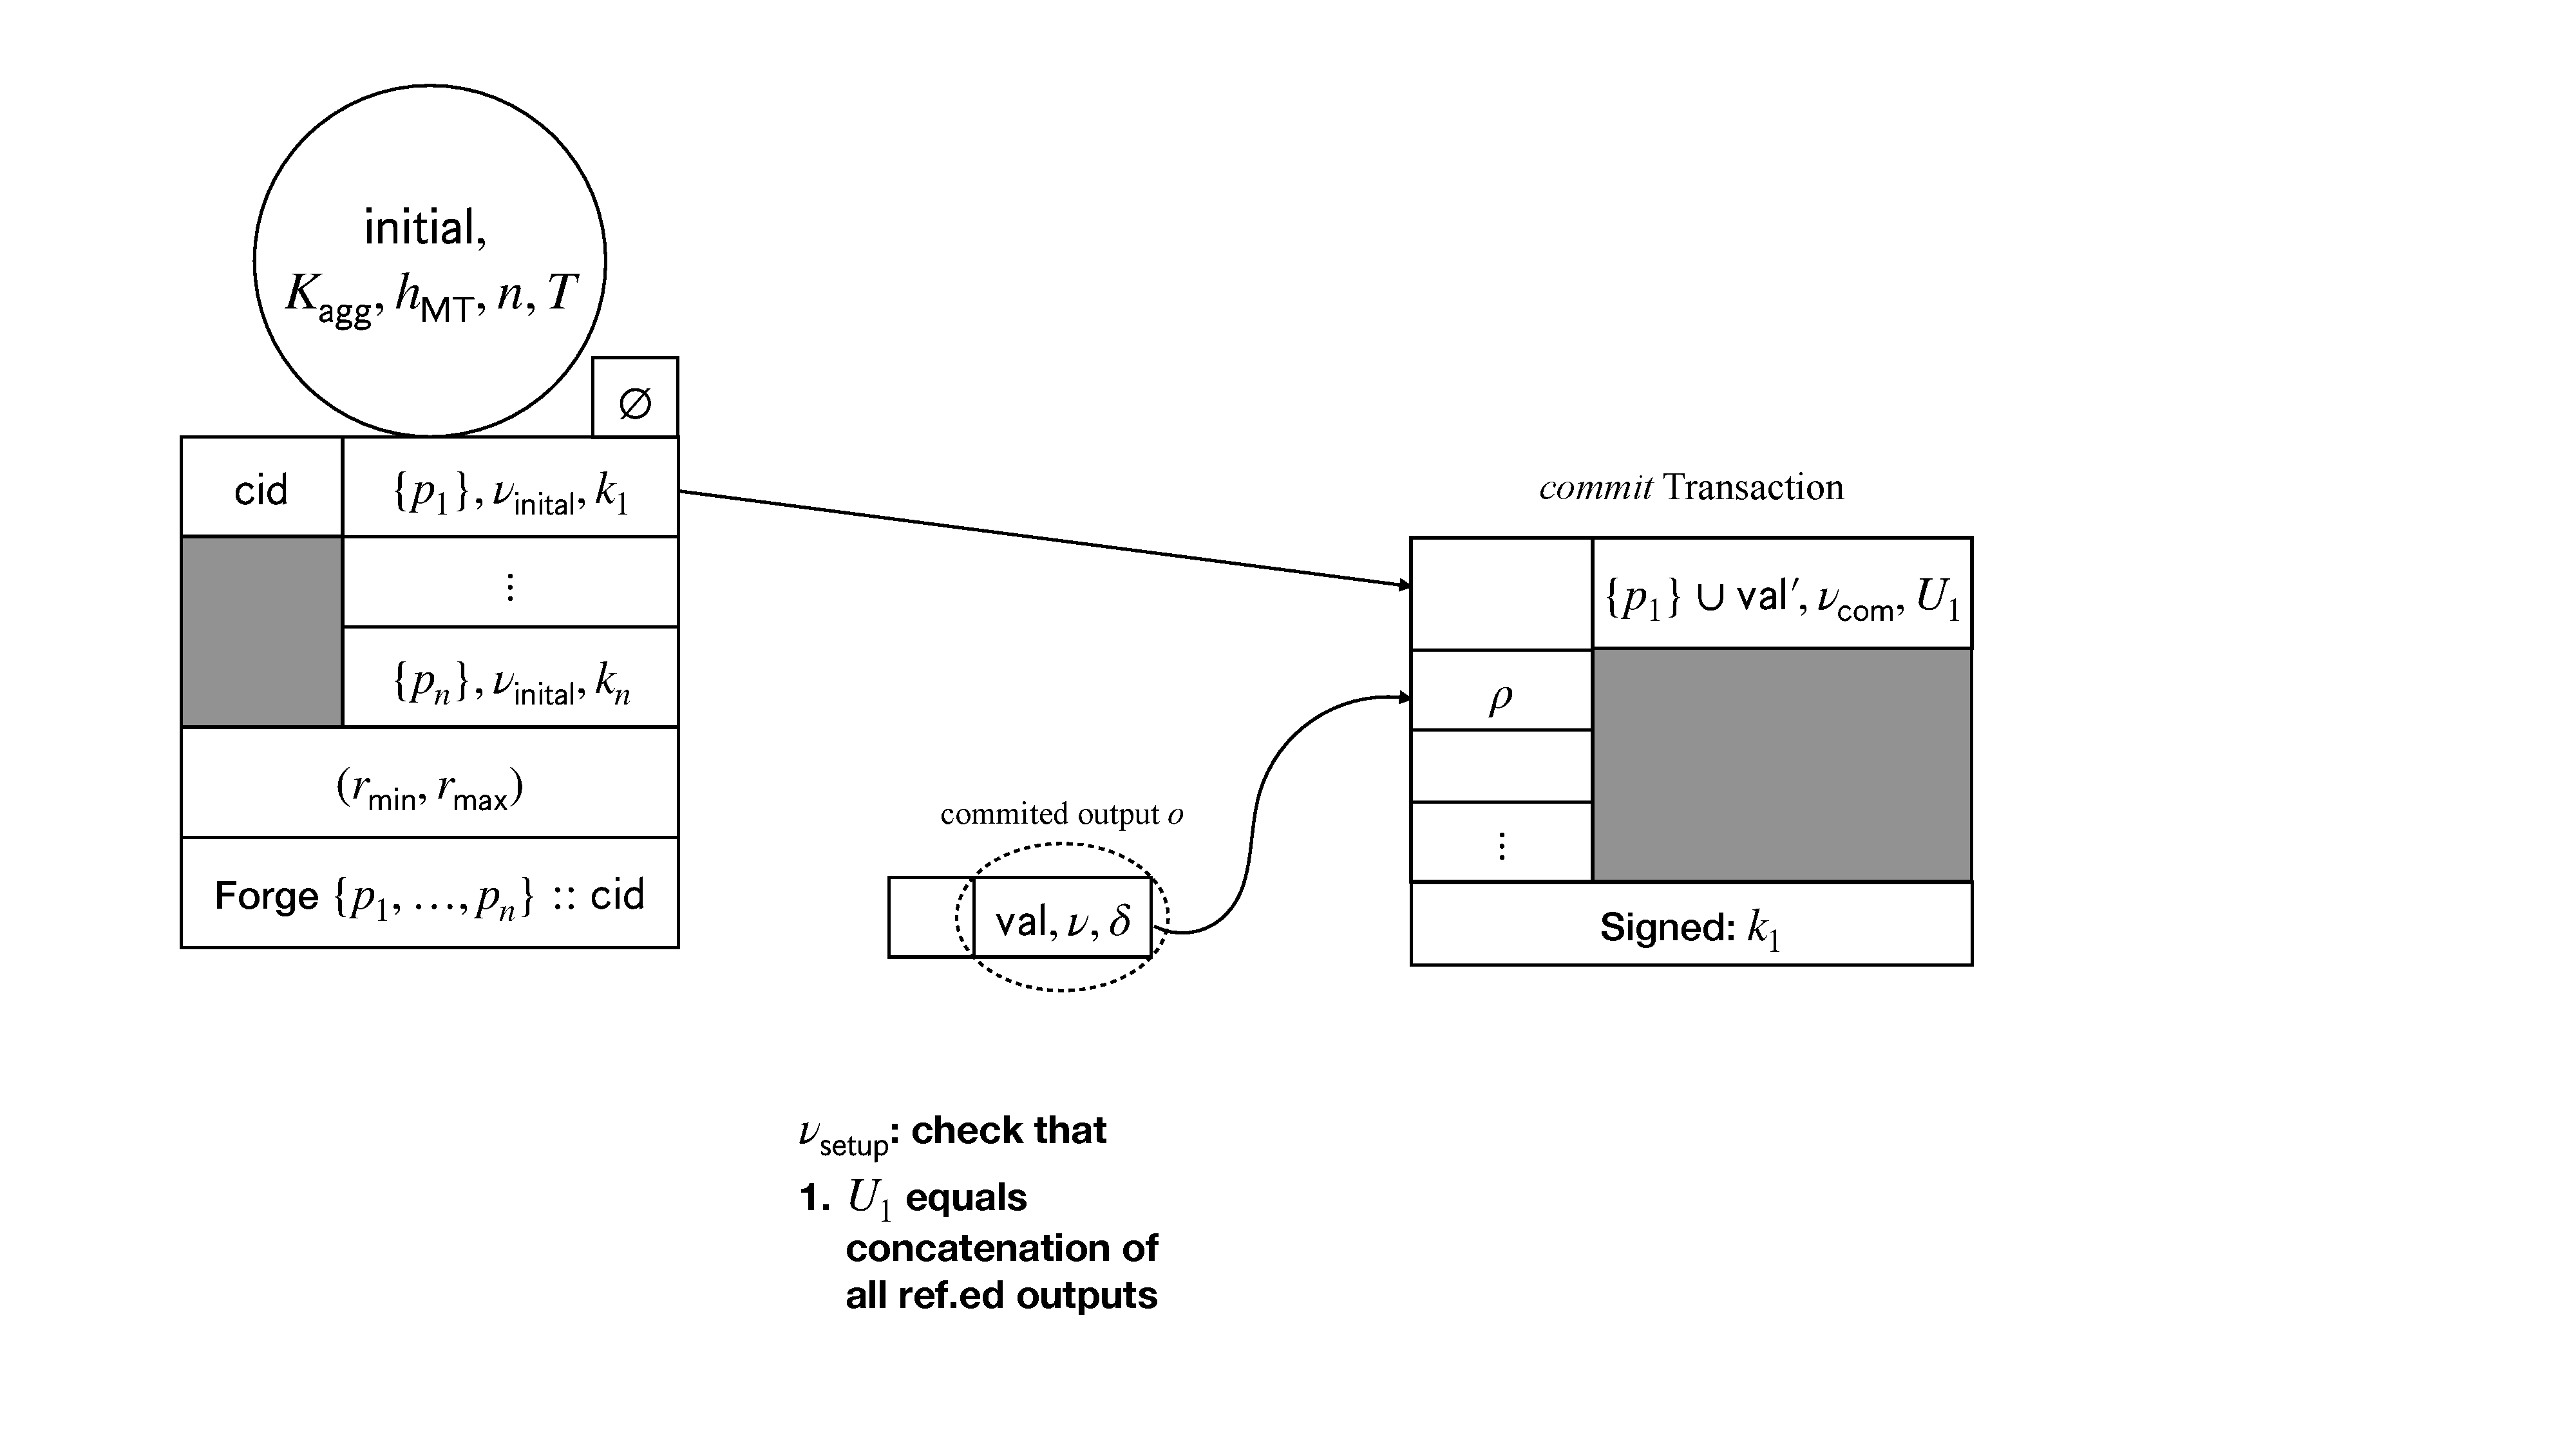
\includegraphics[width=\textwidth/2,trim=130 330 430 50,clip]{figures/SM_commit_tx.pdf}

  % TODO: clean draw marked up version
  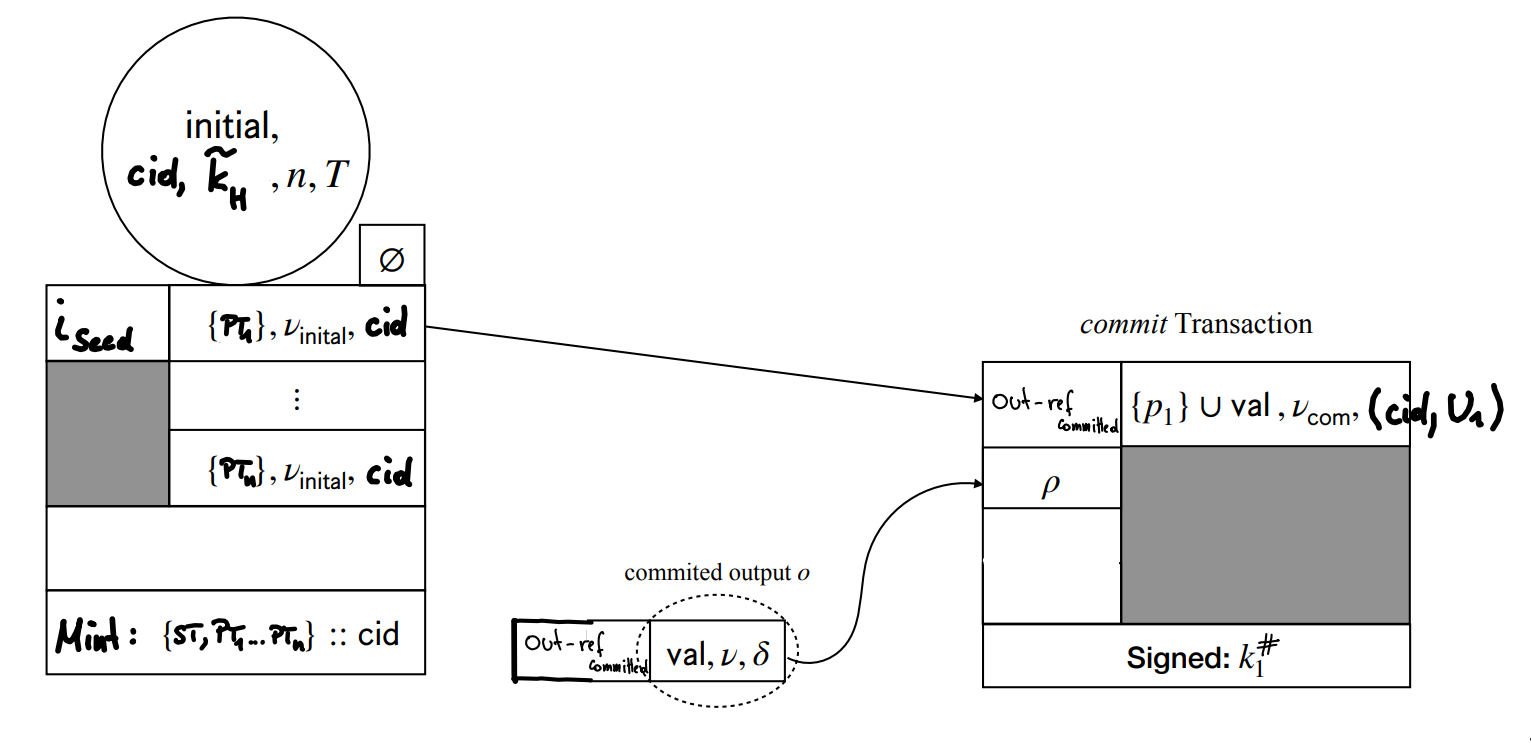
\includegraphics[width=\textwidth*2/3]{figures/SM_commit_tx.png}

  \caption{
    \mtxInit{} transaction (left) with one \mtxCom{} transaction
    (right) attached locking one output (center).}\label{fig:SM_commit_tx}

\end{figure}


%%% Local Variables:
%%% mode: latex
%%% TeX-master: "main"
%%% End:


A \mtxCom{} transaction consumes one $\nuInitial$ UTxO and zero or one \emph{committed} UTxO, and has one output locked by validator $\nuCom$.

\noindent The $\nuInitial$ validator ensures the transaction has the following structure:
\begin{menumerate}
    \item the transaction is signed with verification key corresponding to the asset name in $\mathsf{PT}_i$,
    \item the redeemer for $\nuInitial$ is referencing the output to commit $ \rho = \txOutRef_{commit}$, with output $o_{commit}$ holding value $\val_{commit}$
    \item the committed value is in the output $\val' = \{\mathsf{PT}_{i}\} \cup \val_{commit} $,
    \item the data field $\delta$ of the output locked by $\nuCom$ is $(\mathsf{cid}, U)$ with:
    \begin{menumerate}
        \item $U = \recordUTxO(\txOutRef_{commit},o_{commit})$, and 
        \item $\recordUTxO (\txOutRef, o) = (\txOutRef, \bits(o))$,
    \end{menumerate}        
    \item no minting or burning happens.
\end{menumerate}

\noindent The $\nuCom$ validator ensures the output is collected by either a \mtxCCom{} or \mtxAbort{} transaction.
\begin{boxM}
The \mtxCom{} transaction does not take part in the state machine logic.
\end{boxM}

\subsection{CollectCom Transaction}

\begin{figure}[h]

  \centering

  % 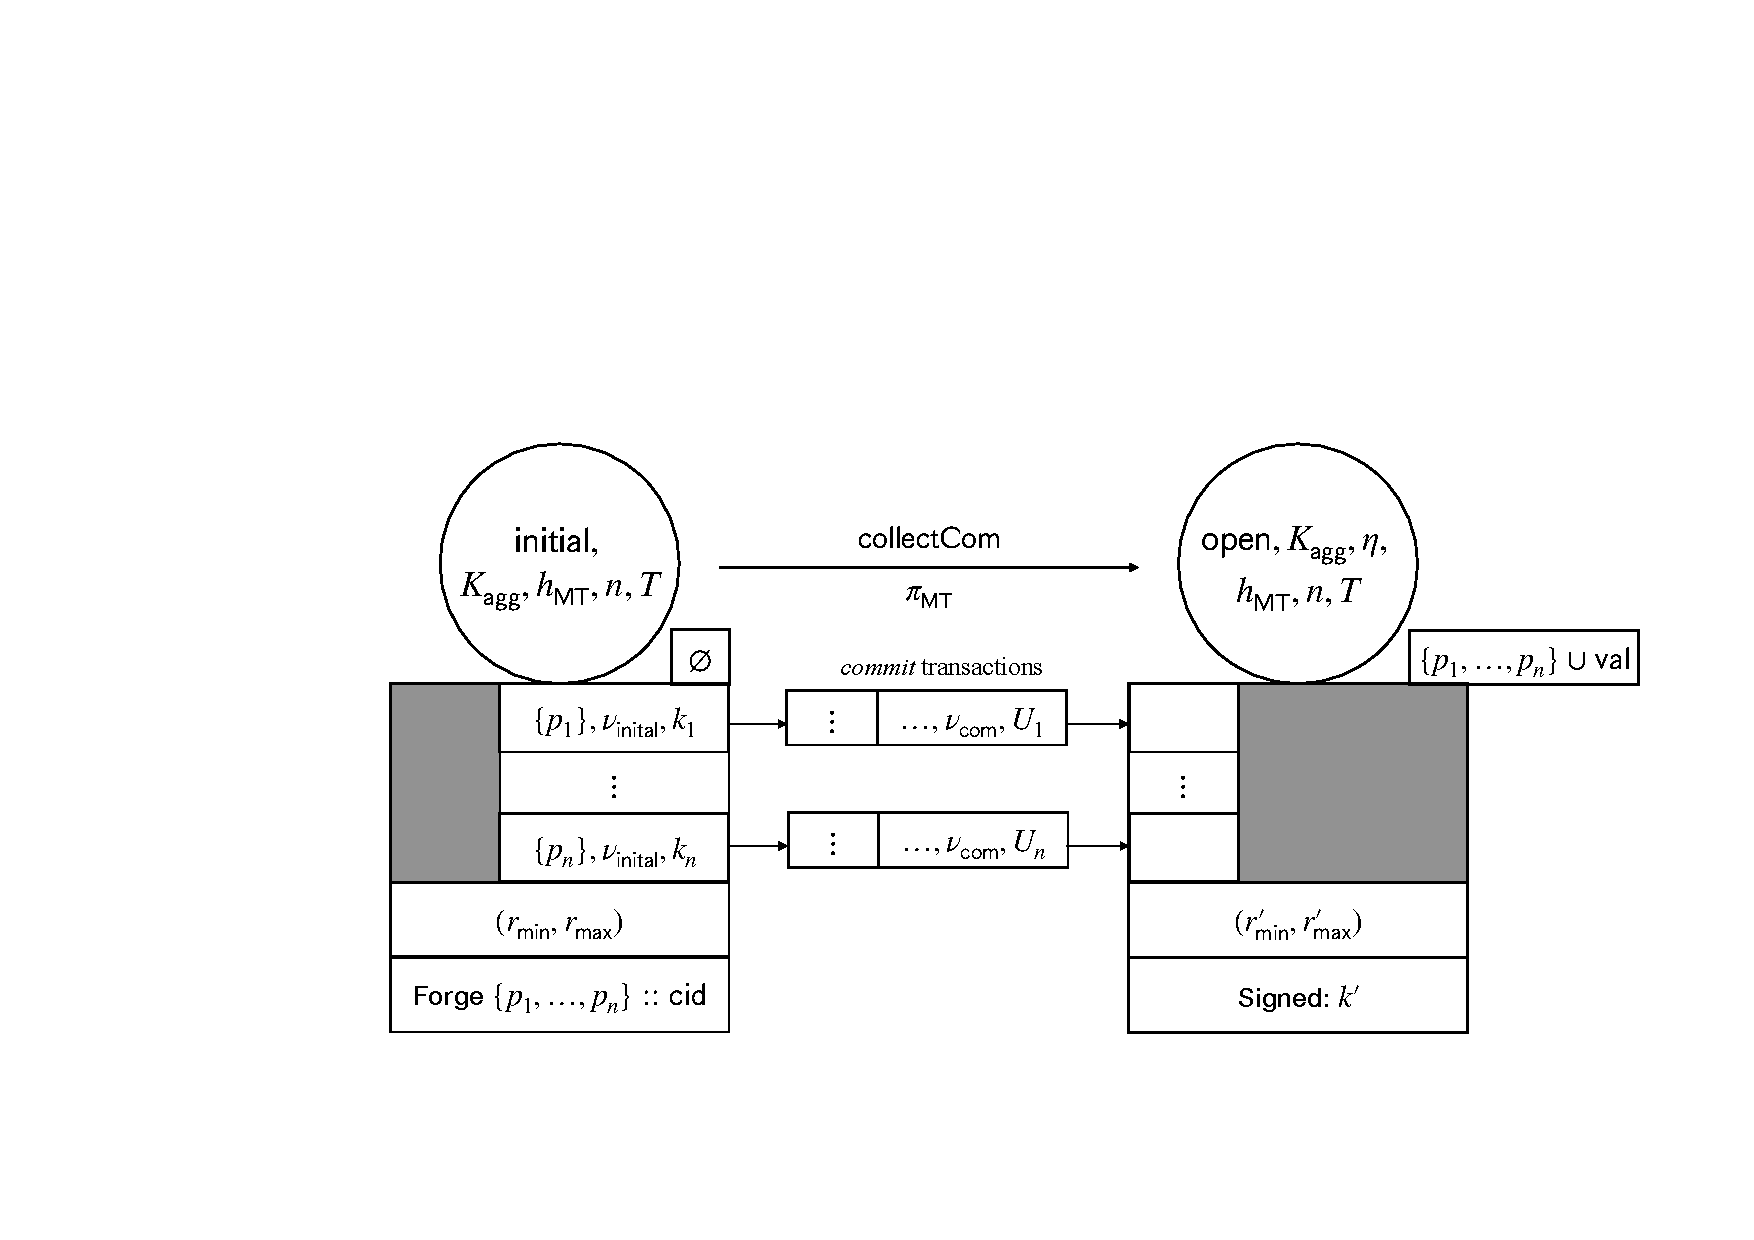
\includegraphics[width=\textwidth/2]{figures/SM_initial_open.pdf}
  %
  % TODO: clean draw marked up version
  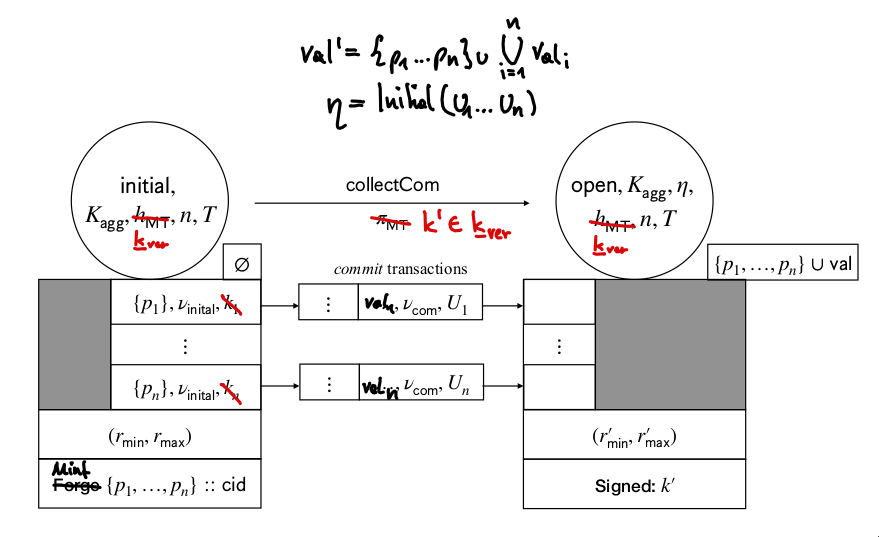
\includegraphics[width=\textwidth/2]{figures/SM_initial_open.png}

  \caption{\mtxInit{} transaction (left) with \mtxCCom{} transaction
    (right) and \mtxCom{} transactions (center).}
  \label{fig:SM_initial_open}

\end{figure}



%%% Local Variables:
%%% mode: latex
%%% TeX-master: "main"
%%% End:


The \mtxCCom{} transaction collects all outputs from \mtxCom{} transactions participating in the same head and advances the state of the CEM state machine
$$
   (\stInitial,\hpAK,\hppuv,\nop,\cPer) \xrightarrow{\mathsf{collectCom}} (\stOpen,\hpAK,\eta,\hppuv,\nop,\cPer),
$$
where
$$
\eta = \mathsf{Combine}(U_{1}, \ldots, U_{n}).
$$

The $\nuHead$ validator additionally checks that:
\begin{menumerate}
  \item all committed value captured and no additional funds ``enter'' or ``leave''
  $\val' = \bigcup_{i=1}^{n} \mathsf{PT}_{i} \cup \val_{i}$,
  \item all tokens present in output
  $|\{cid \rightarrow . \rightarrow 1\} ~ \mathsf{in} ~ \val'| = \nop + 1$,
  \item the transaction is signed by a verification key $k' \in \hppuv$ with its
  hash corresponding to the asset name of one of the participation tokens
  $\{p_1 \dots p_n\}$,
  \item unchanged parameters $\mathsf{cid}$, $\hpAK$, $\hppuv$, $\nop$, and
  $\cPer$ in the data field,
  \item no minting or burning happens.
\end{menumerate}

\noindent Each of the $\nuCom^i$ validators, for $i \in \{ 1\dots n\}$, checks:
\begin{menumerate}
    \item the ST token is present in the output value $\{cid \rightarrow ST \rightarrow 1\} \subseteq \val'$
    \item with the correct $\mathsf{cid}$ in the datum $(cid,.) = \delta$.
\end{menumerate}

\subsection{Abort Transaction}\label{sec:abort-tx} 

\begin{figure}

  \centering

  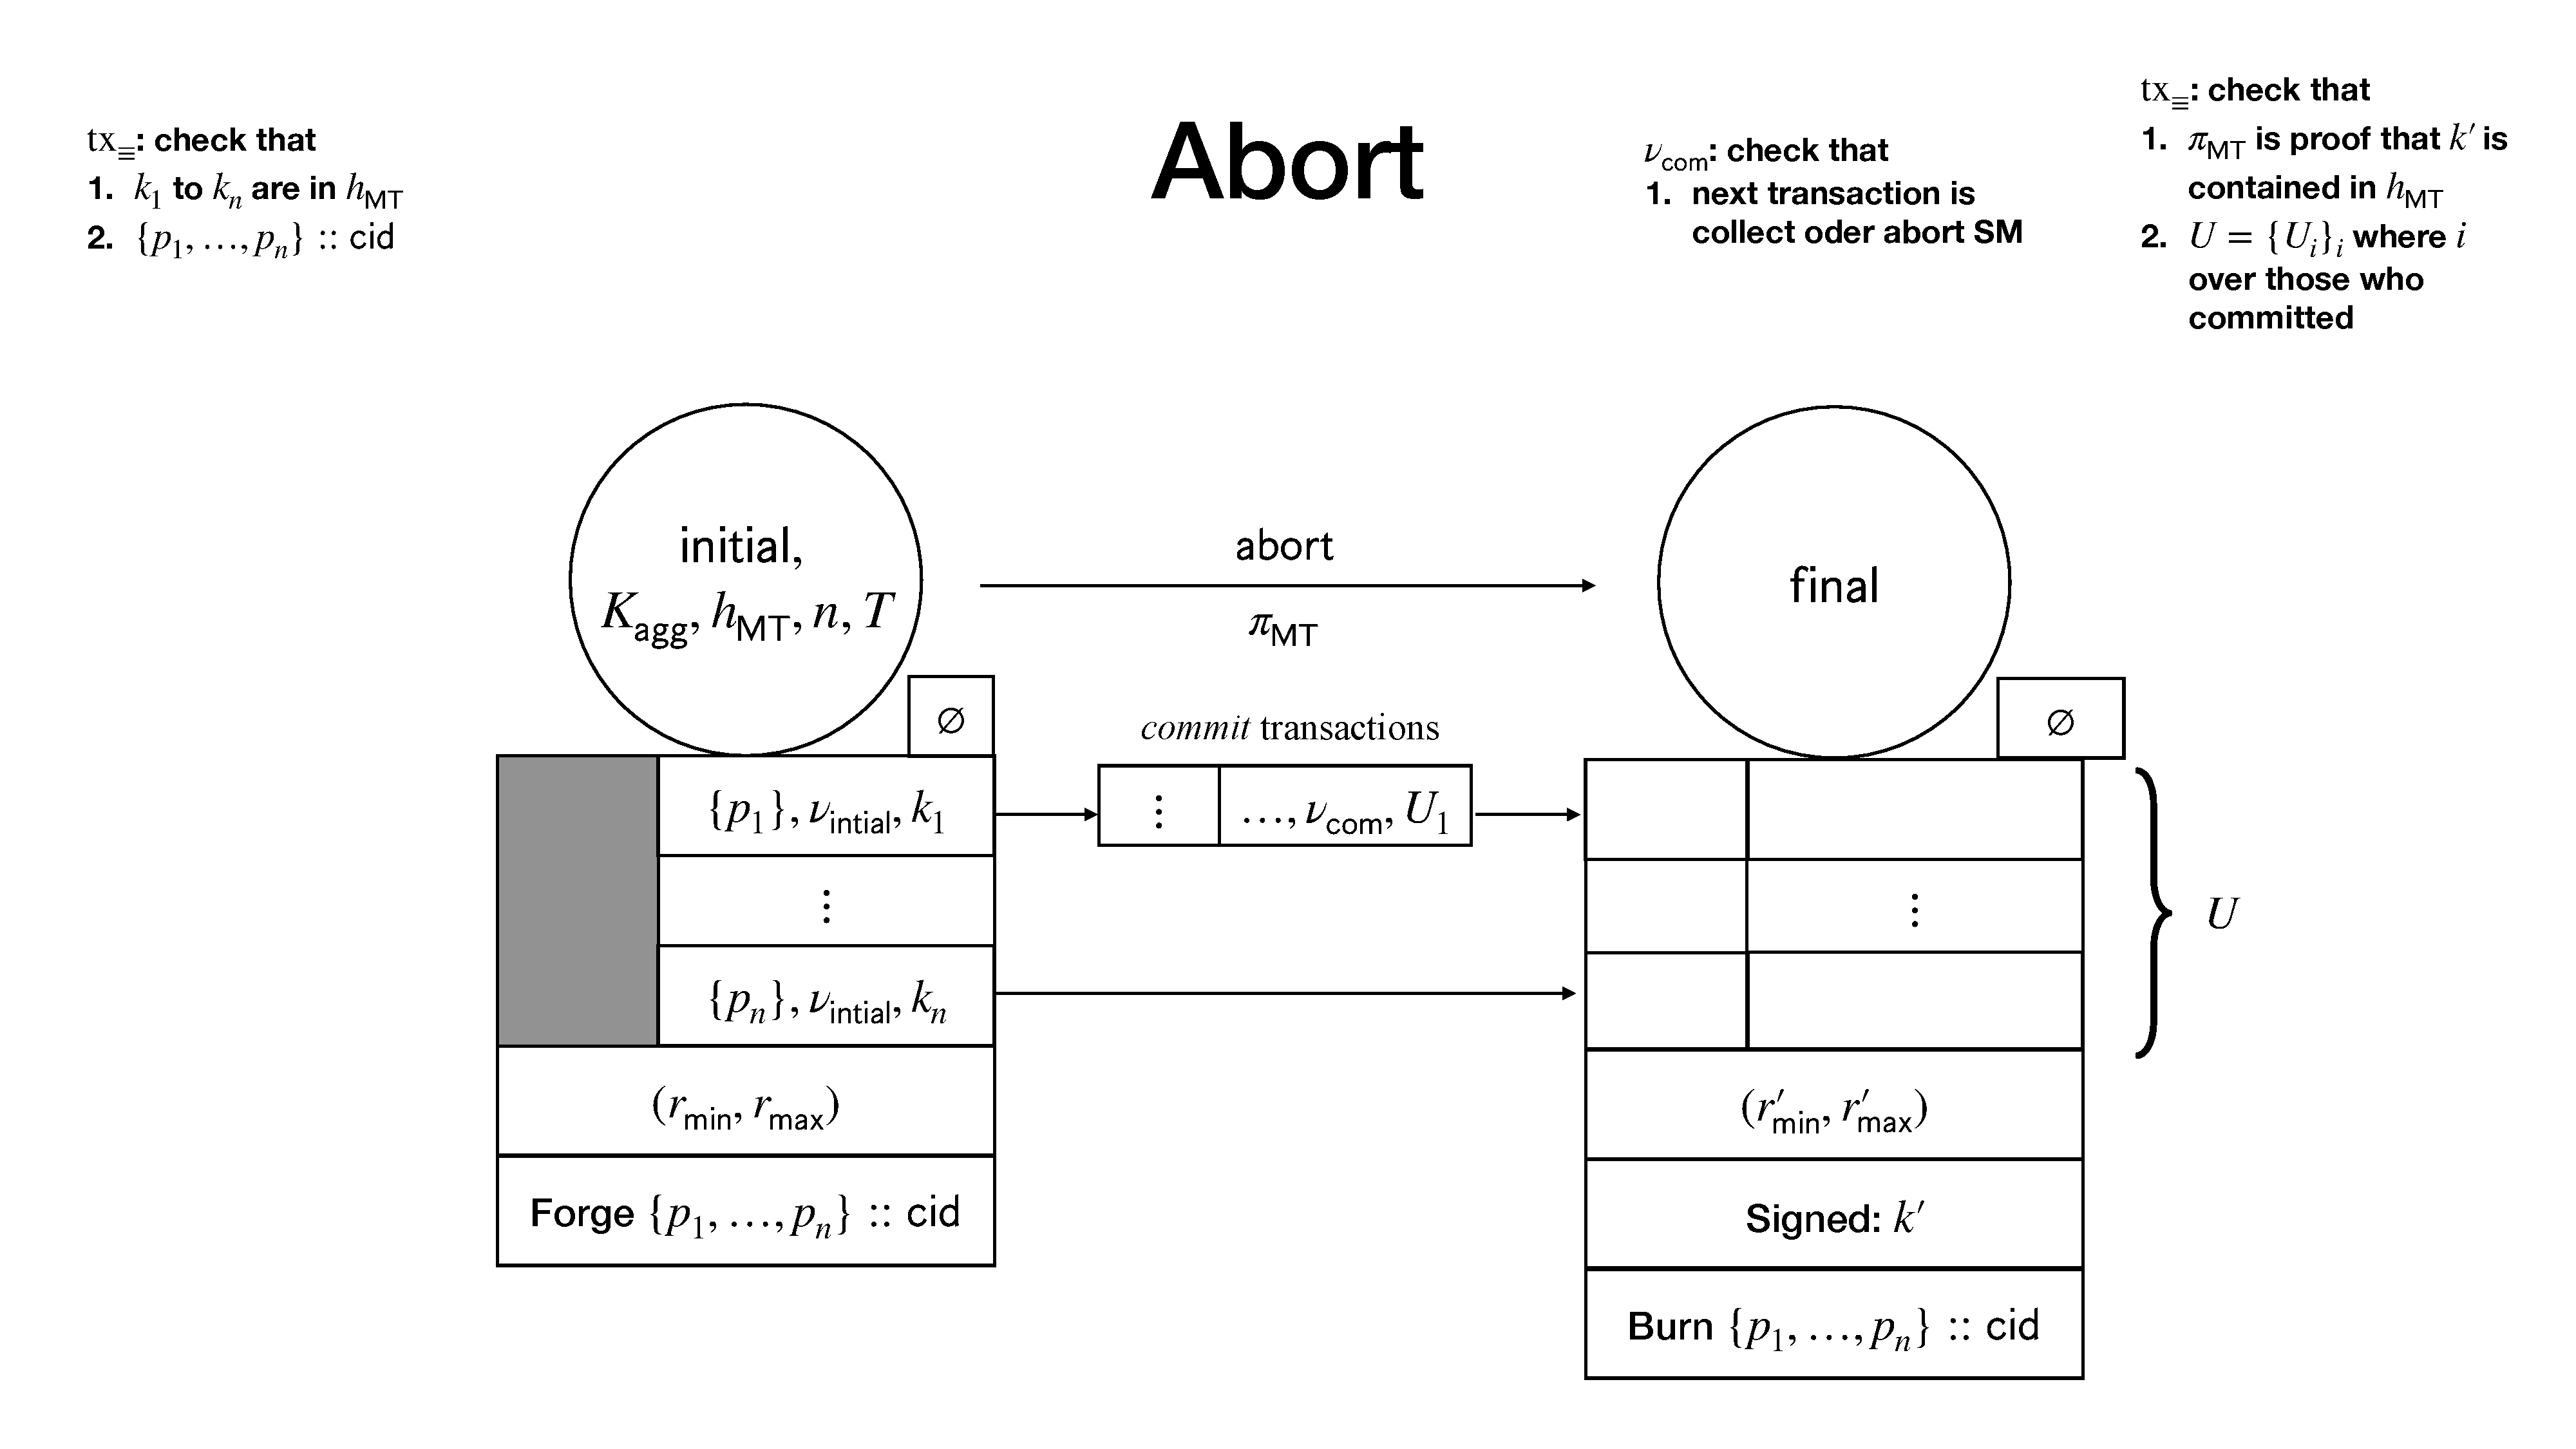
\includegraphics[width=\textwidth/2-2em,trim=350 20 240 300,
  clip]{figures/SM_initial_final.pdf}
    
  \caption{\mtxInit{} transaction (left) with \mtxAbort{} transaction
    (right) and \mtxCom{} transactions (center).}
  \label{fig:SM_initial_final}

\end{figure}



%%% Local Variables:
%%% mode: latex
%%% TeX-master: "main"
%%% End:


The \mtxAbort{} transaction
(see Fig.~\ref{fig:SM_initial_final}) allows a party to abort the
creation of a head.  The state is transitioned to $\mathsf{final}$ and the $\nuHead$ validator ensures that:
\begin{menumerate}
 \item All outputs committed into the head are recreated as is: $\forall i \in \{1\dots\nop\}, \mathcal{H}(O[i]) = \delta_i$,
 \item All participation tokens are burnt: $\forall i \in \{1\dots\nop\}, \{\mathsf{cid} \rightarrow \mathsf{PT}_i \rightarrow -1\} \subseteq Mint.$
\end{menumerate} 

\noindent For each of the $\nuInitial$ validators consumed, checks:
\begin{menumerate}
  \item The data field $\delta$ of the output locked is $(\mathsf{cid}$,
  \item The ST token is getting burned $\{cid \rightarrow ST \rightarrow -1\} \subseteq \mathsf{Mint}.$ 
\end{menumerate}

\noindent For each of the $\nuCom$ validators consumed, checks:
\begin{menumerate}
  \item The ST token is getting burned $\{cid \rightarrow ST \rightarrow -1\} \subseteq \mathsf{Mint}$
  \item The correct $\mathsf{cid}$ is in the datum $(cid,.) = \delta$.
\end{menumerate}

\subsection{Close Transaction} 

In order to close a head, a head
member may post the \mtxClose{} transaction (see
Fig.~\ref{fig:SM_open_closed}), which results in a SM transition
from the $\stOpen$ state to the $\stClosed$ state.
\\
\\
Performed $\nuHead$ validator checks:

\begin{enumerate}
  \item Verify off-chain signatures on a snapshot or keep recorded UTxO data unchanged if there is no snapshot 
  \item Record contestation deadline: at least $L$ time after close transaction and ensure $Tmax - Tmin <= L$ 
  \item Record public key hash of participant who posts in a set C
  \item Value preservation
  \item Nothing minted or burned
\end{enumerate}

\noindent Off-chain transaction construction needs to make sure that the transaction validity is well bounded and it can be at most $L$ time.
\\
\\
Once a \mtxClose{} transaction has been posted, a \emph{contestation period}
begins which should last for $L$ time. Hence, the deadline is recorded in the state, and it is bounded such that $Tmax - Tmin \leq L$.
\\
\\
Finally, the SM state is extended by a set $\contesters$
initialized to the poster's signing key, i.e.,
$\contesters \gets \{k'\}$.   $\contesters$ is used to ensure that no party
posts more than once during the contestation period.


\begin{figure}[t!]

  \centering

  %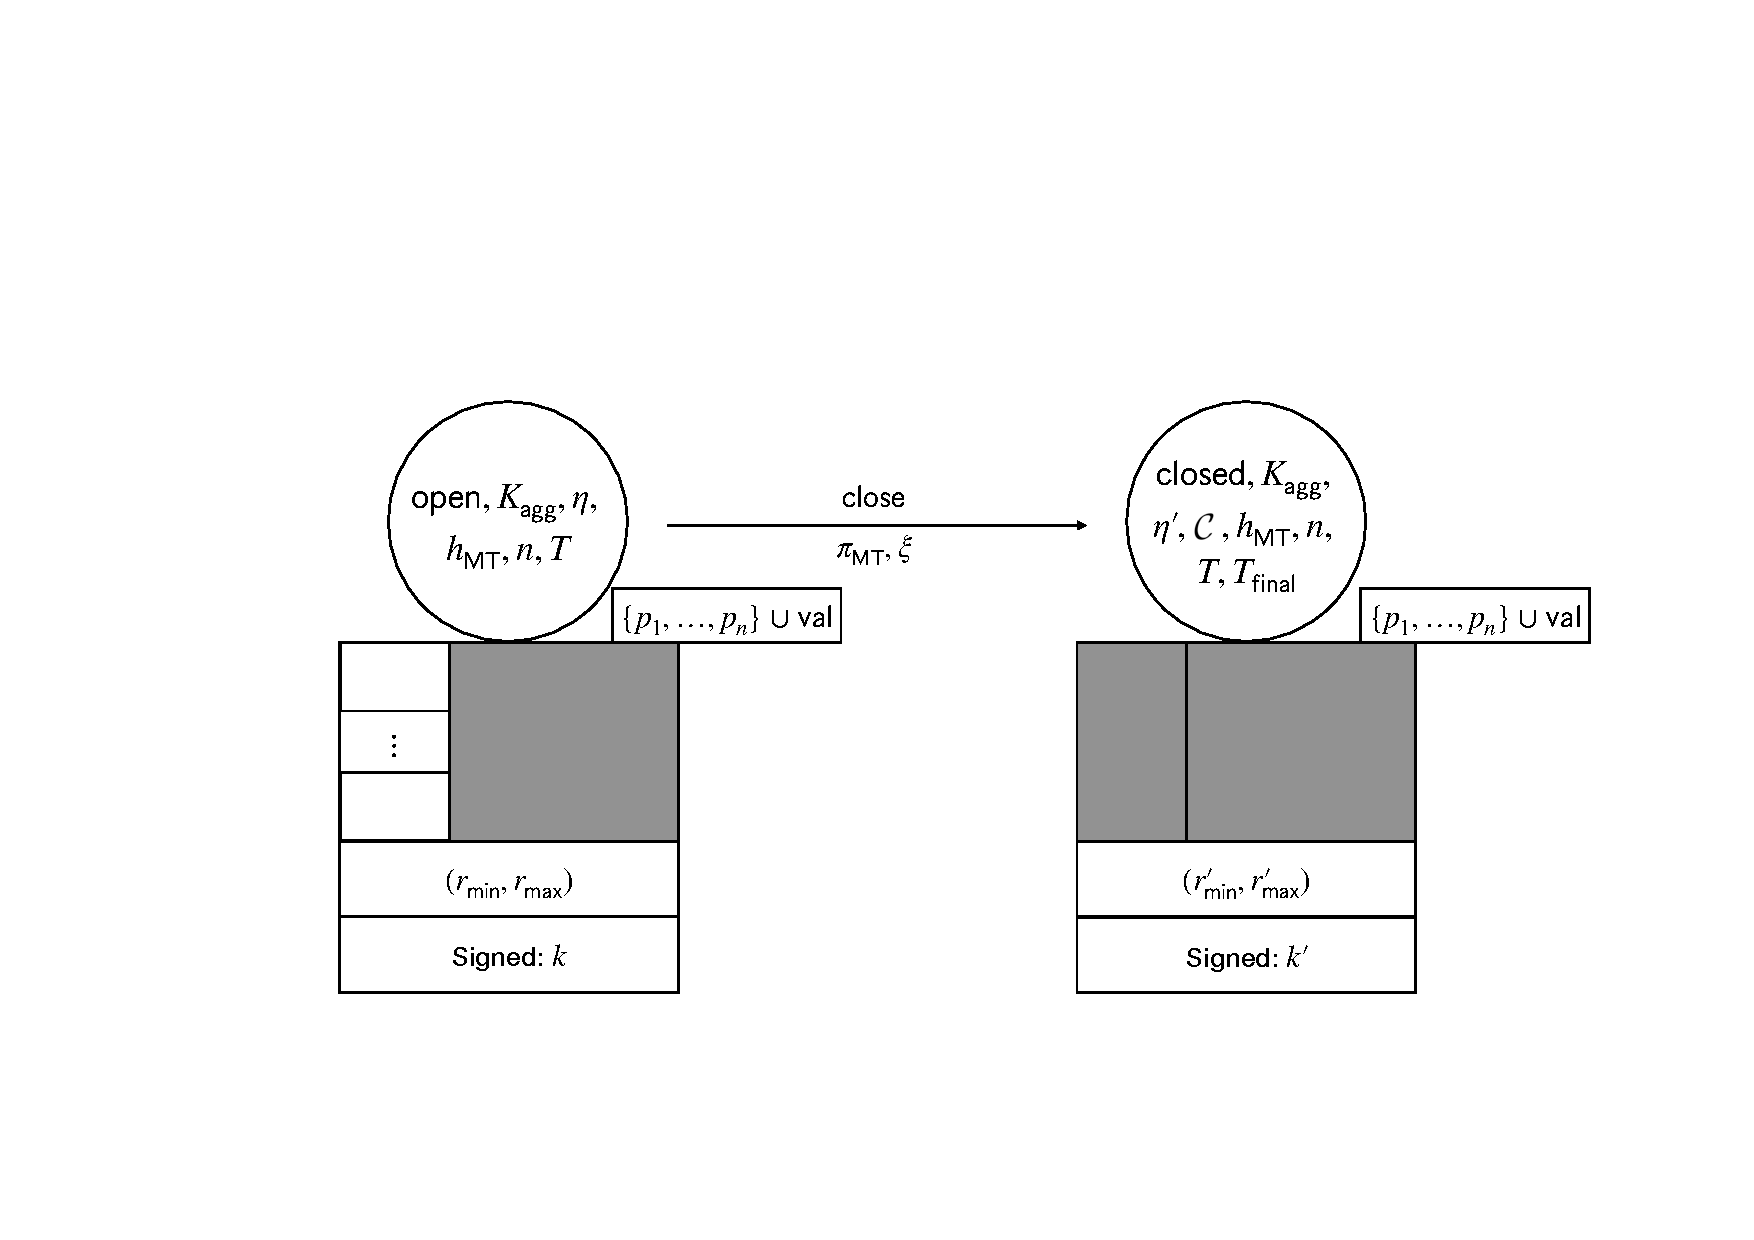
\includegraphics[width=\textwidth/2-2em,trim=350 100 160 300,
  %clip]{figures/SM_open_closed.pdf}

  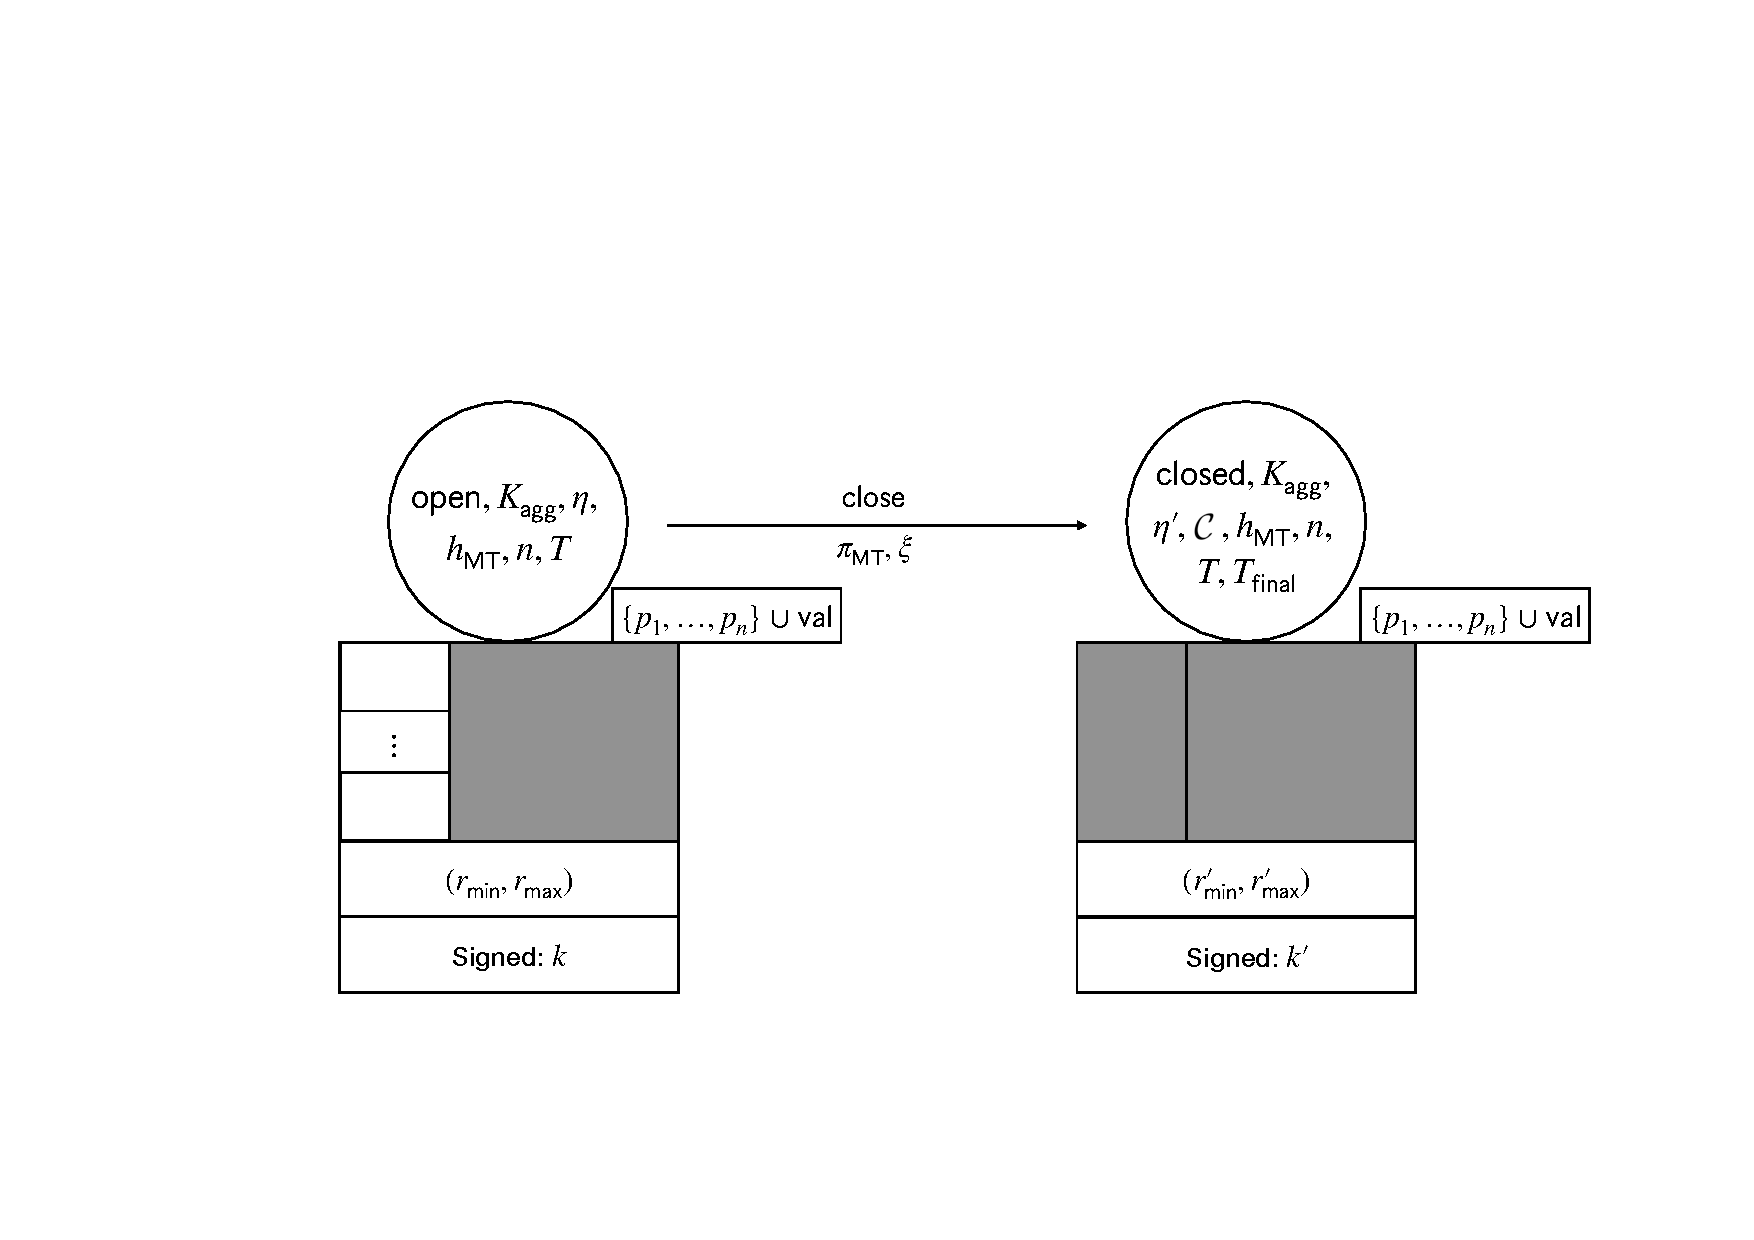
\includegraphics[width=\textwidth/2]{figures/SM_open_closed.pdf}

  \caption{\mtxCCom{} transaction (left) with \mtxClose{}
    transaction (right).}
  \label{fig:SM_open_closed}

\end{figure}



%%% Local Variables:
%%% mode: latex
%%% TeX-master: "main"
%%% End:



\subsection{Contest Transaction} 

The \mtxContest{} transaction (see
Fig.~\ref{fig:SM_closed_closed}) is posted by a party to prove the currently $\stClosed$ state is not the latest one. 

\noindent Performed $\nuHead$ validator checks:
\begin{enumerate}
   \item Verify off-chain snapshot signature
   \item Record contestation deadline: at least L time after this contest
   \item Record public key hash of participant who posts in a set C
   \item Ensure there is no contest by someone in C
   \item Value preservation
   \item Nothing minted or burned
\end{enumerate}

\noindent This causes the following transition in the CEM state machine (eg. change datum of output locked by $\nuHead$ script):
$$
   (\stClosed,\hpAK,\eta,\eta_0,\mathcal{C},\hppuv,\nop,\cPer,\Tfinal) \xrightarrow[\xi]{\mathsf{contest}} (\stClosed,\hpAK,\eta',\eta_0,\mathcal{C}', \hppuv,\nop,\cPer,\Tfinal'),
$$

\noindent The $\nuHead$ validator additionally checks that:
\begin{menumerate}
  \item Value is preserved $\val' = \val$,
  \item The transaction is signed by a verification key $k' \in \hppuv$ with its
  hash corresponding to the asset name of one of the participation tokens
  $\{\mathsf{PT}_1 \dots \mathsf{PT}_\nop\}$,
  \item The signer has not already contested $k' \not\in \mathcal{C},$  and it's added to the signers set: $\mathcal{C}' = \mathcal{C} \cup k',$
  \item $\eta'$ is valid w.r.t. to previous state (see below), 
  \item Transaction is posted before deadline: $T_{\mathsf{max}} \leq \Tfinal$,
  \item Contestation deadline is updated:
     $$
     \Tfinal' = 
        \{\begin{array}{ll}
             \Tfinal     &  |\mathcal{C}'| = n, \\
             \Tfinal + T &  \mathit{otherwise} \\
        \end{array},
     $$
  \item Values for $\hpAK$, $\hppuv$, $\nop$, $\eta_0$, and $\cPer$ are unchanged,
  \item no minting or burning happens.
\end{menumerate}

\subsubsection{Contested State Verification}

The $\nuHead$ validator uses auxiliary function $\mathsf{VerifyMultiSignature}$ to check that $\xi$ is 
$$
\xi = (s,U, \mathsf{sig})
$$

The transition handles update
information $\xi$ by passing it through OCV algorithm $\ocvContest$,
resulting in a new OCV status
$\eta' \gets \ocvContest (\hpAK,\eta,\xi)$.  OCV algorithm
$\ocvContest$ uses the previous OCV status $\eta$ and $\hpAK$ to check
the update information $\xi$.  Similarly to $\ocvClose$, $\ocvContest$
may output $\bot$, but in order for a \mtxContest{} transaction to be
valid $\eta' \neq \bot$ is required.

The \mtxContest{} transaction is only valid if the old set
$\contesters$ of parties who have contested (or closed) so far does not yet
include the poster, i.e., $k' \notin \contesters$.  If this check
passes, the set is extended to include the poster of the \mtxContest{}
transaction, i.e., $\contesters' \gets \contesters \cup \{k'\}$.
Furthermore, \mtxContest{} transactions may only be posted up until
$\Tfinal$, i.e., it is required that $\txRmax' \leq \Tfinal$.

Observe that during the contestation period, up to $\nop-1$
\mtxContest{} transactions may be posted (of course, the parameter
$\cPer$ has to be chosen large enough as to allow each head member to
potentially post a \mtxClose{}/\mtxContest{} transaction).


\begin{figure}

  \centering

  %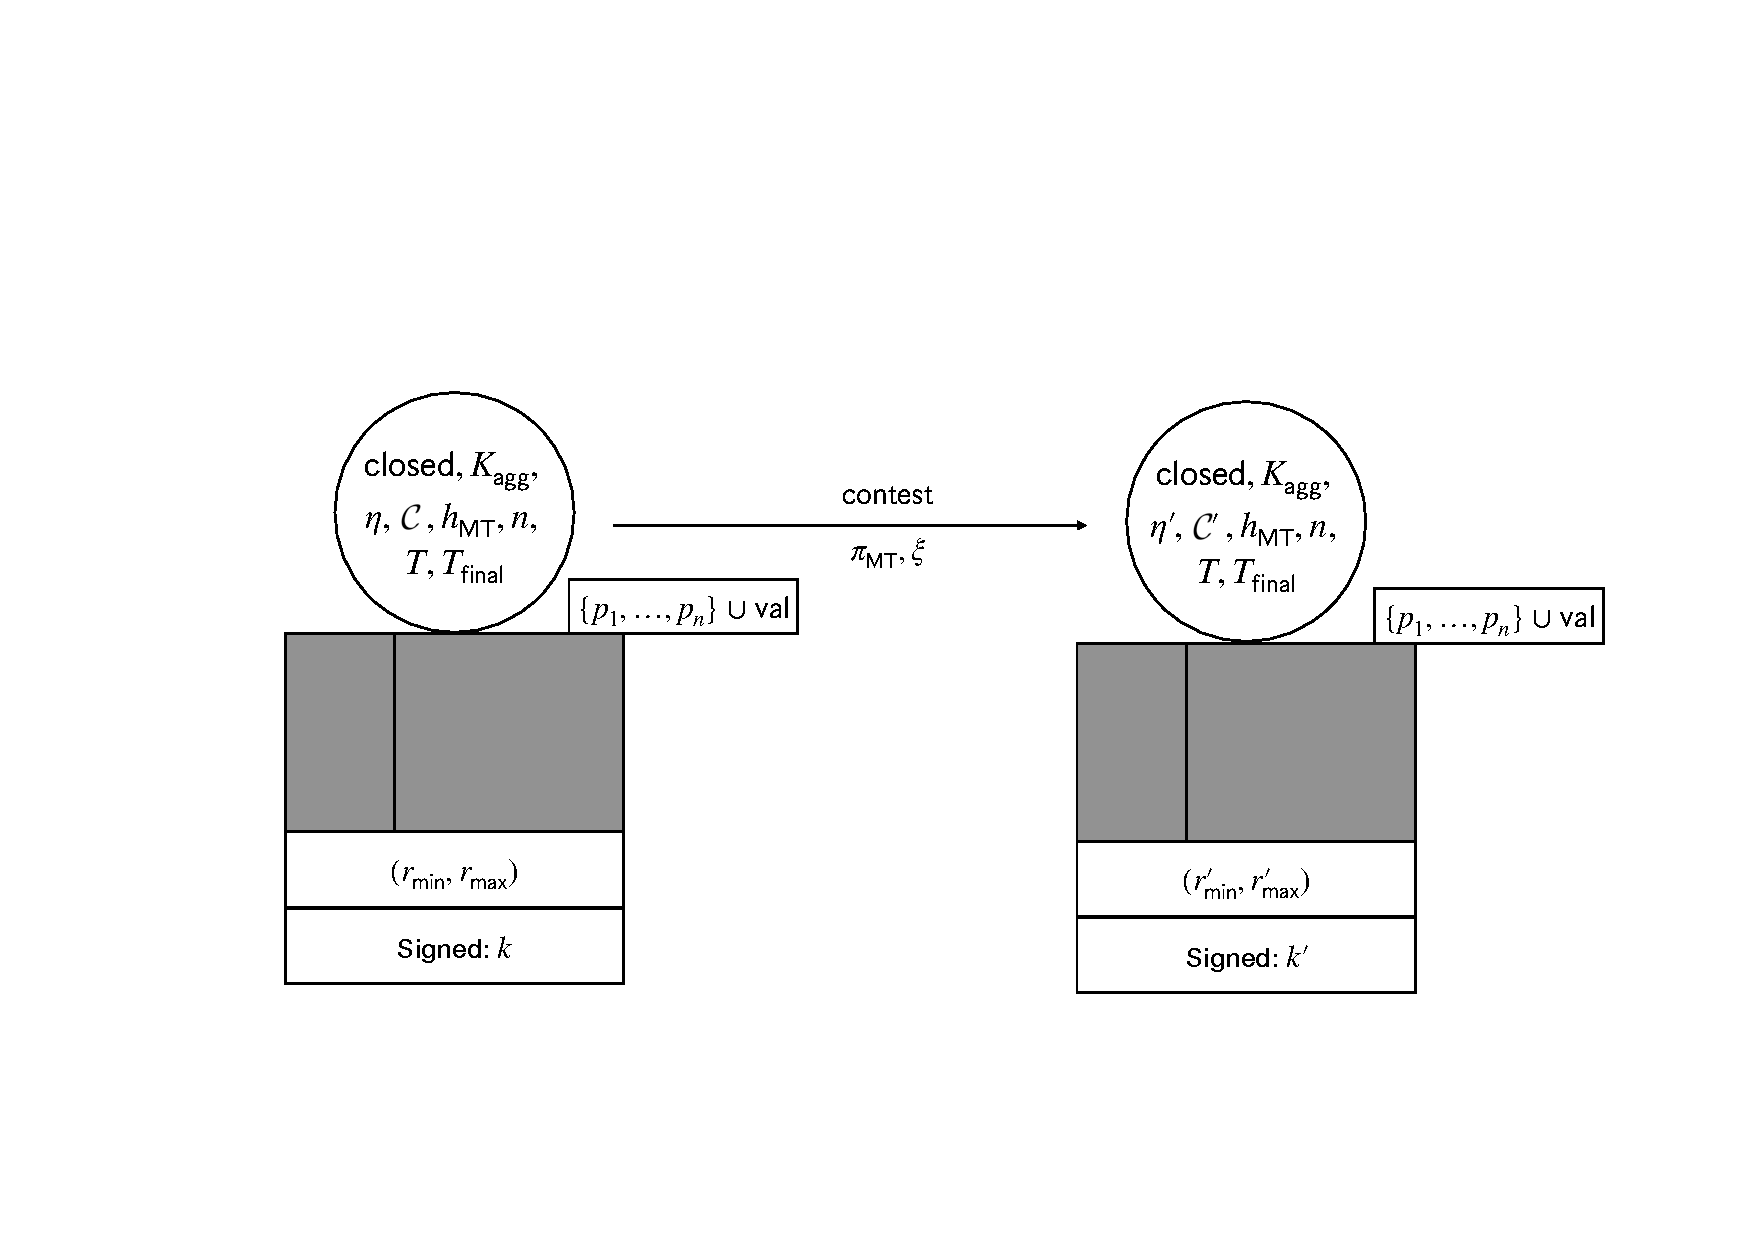
\includegraphics[width=\textwidth/2-2em,trim=280 120 160 260,
  %clip]{figures/SM_closed_closed.pdf}

  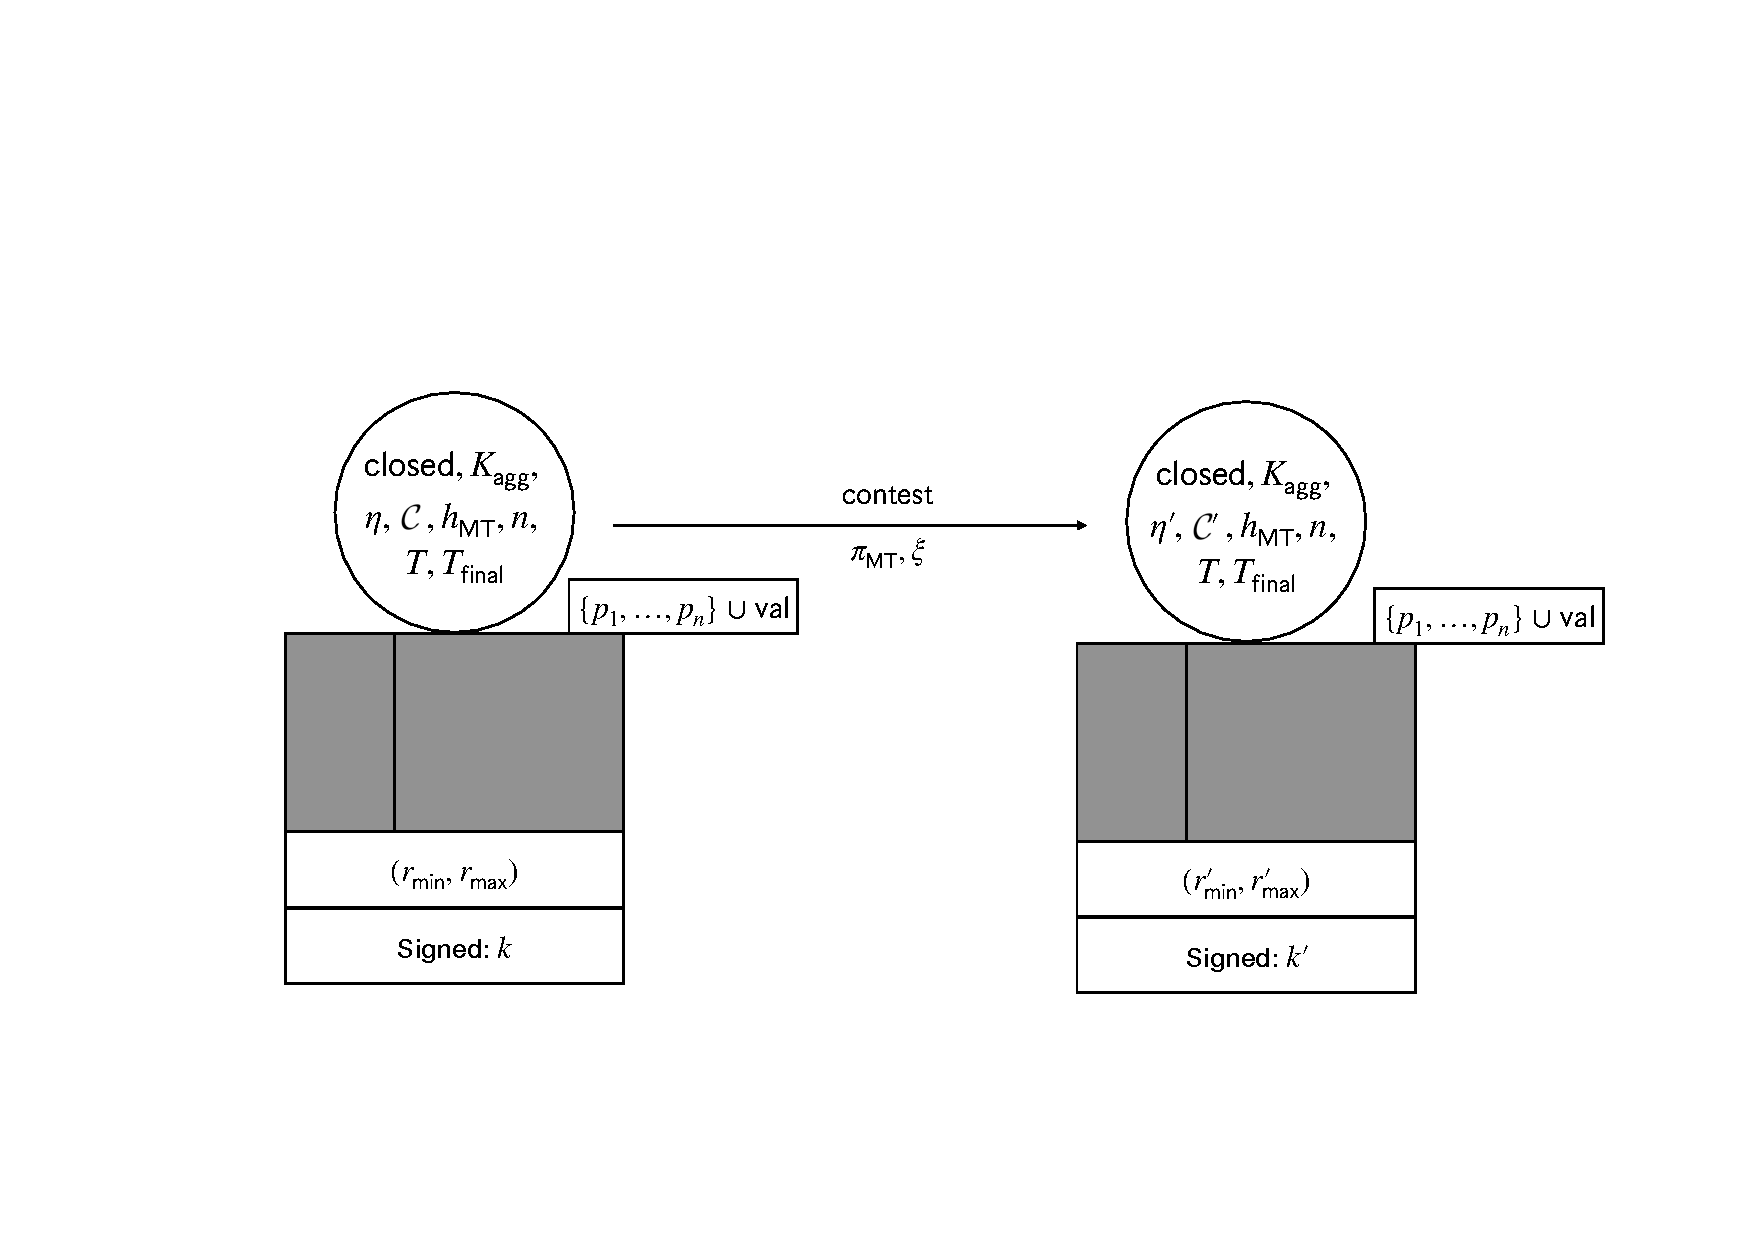
\includegraphics[width=\textwidth/2]{figures/SM_closed_closed.pdf}

  \caption{\mtxClose{}/\mtxContest{} transaction (left);
    \mtxContest{} transaction (right)}
  \label{fig:SM_closed_closed}

\end{figure}



%%% Local Variables:
%%% mode: latex
%%% TeX-master: "main"
%%% End:


\begin{figure}

  \centering

  % 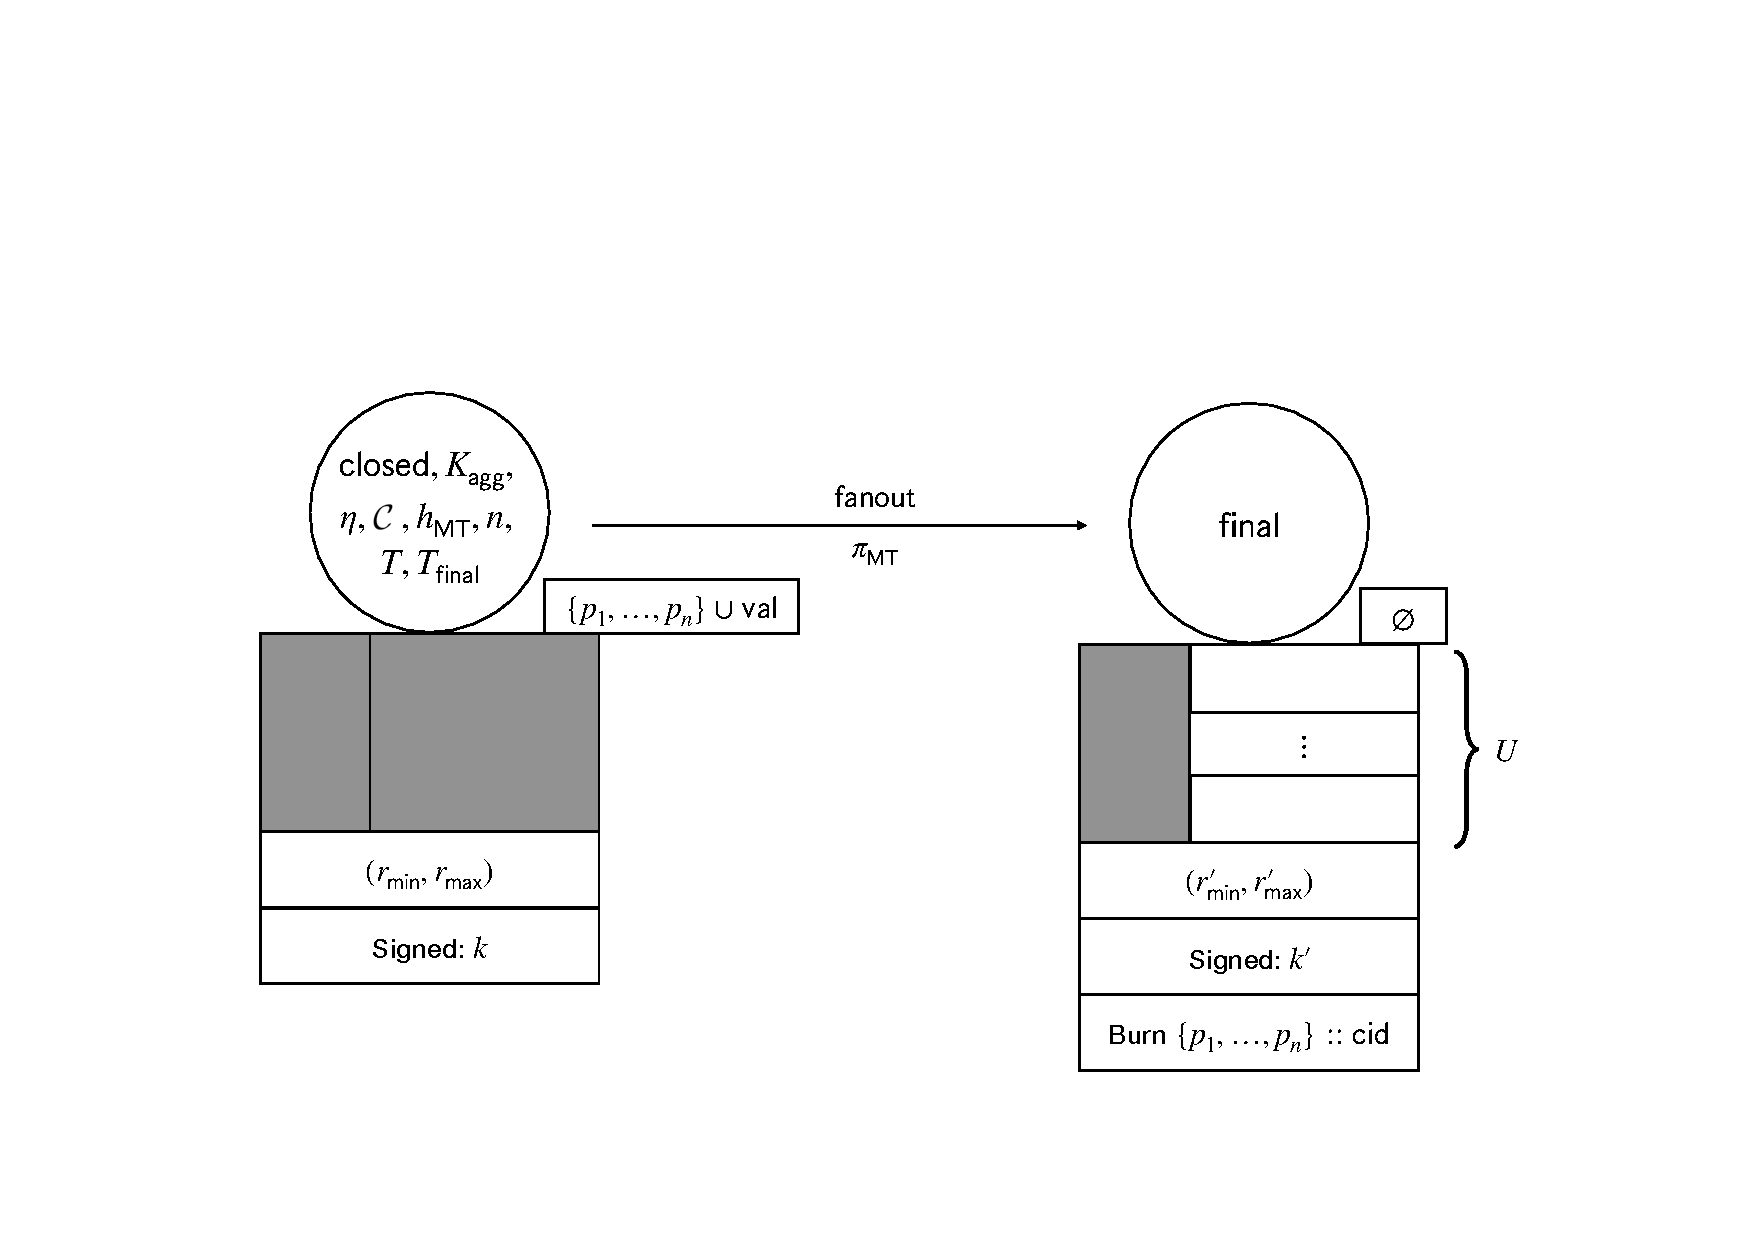
\includegraphics[width=\textwidth/2]{figures/SM_closed_final.pdf}

  % TODO: clean draw marked up version
  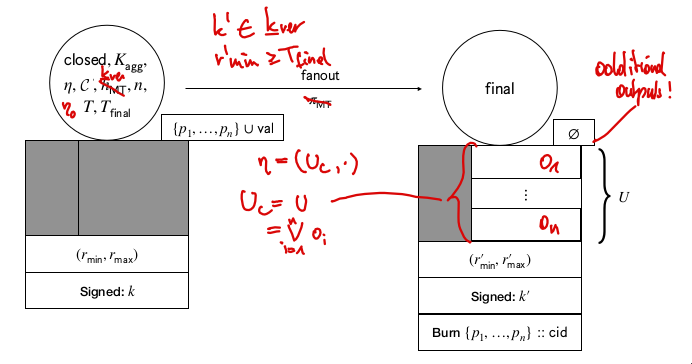
\includegraphics[width=\textwidth/2]{figures/SM_closed_final.png}

  \caption{\mtxClose{}/\mtxContest{} transaction (left);
    \mtxFanout{} transaction (right)}\label{fig:SM_closed_final}

\end{figure}

%%% Local Variables:
%%% mode: latex
%%% TeX-master: "main"
%%% End:


\subsection{Fan-Out Transaction}  

Once the contestation phase is over, a head
may be finalized by posting a \mtxFanout{} transaction, taking the SM
from $\stClosed$ to $\stFinal$.  The \mtxFanout{} transaction must
have outputs that correspond to the most recent head state. 
\newline
\newline 
Performed $\nuHead$ validator checks:
\begin{enumerate}
  \item Correct outputs are created
  \item All tokens are burned
\end{enumerate}

\noindent To that end, $\nuHead$ validator checks the transaction's output set $U$
against the information recorded in $\eta$. To ensure that the \mtxFanout{} transaction is not posted too early,
$\txRmin' > \Tfinal$ is required.  Finally, all participation tokens
must be burned.


%%% Local Variables:
%%% mode: latex
%%% TeX-master: "main"
%%% End:
